\section{lemma6}
\begin{lemma}
\end{lemma}
Suppose we have a local braid diagram and a sheaf singular supported along the braids represented by the following:

\begin{figure}[H] % Optional: [h] means here, [t] for top, [b] for bottom, [p] for page of floats
    \centering
    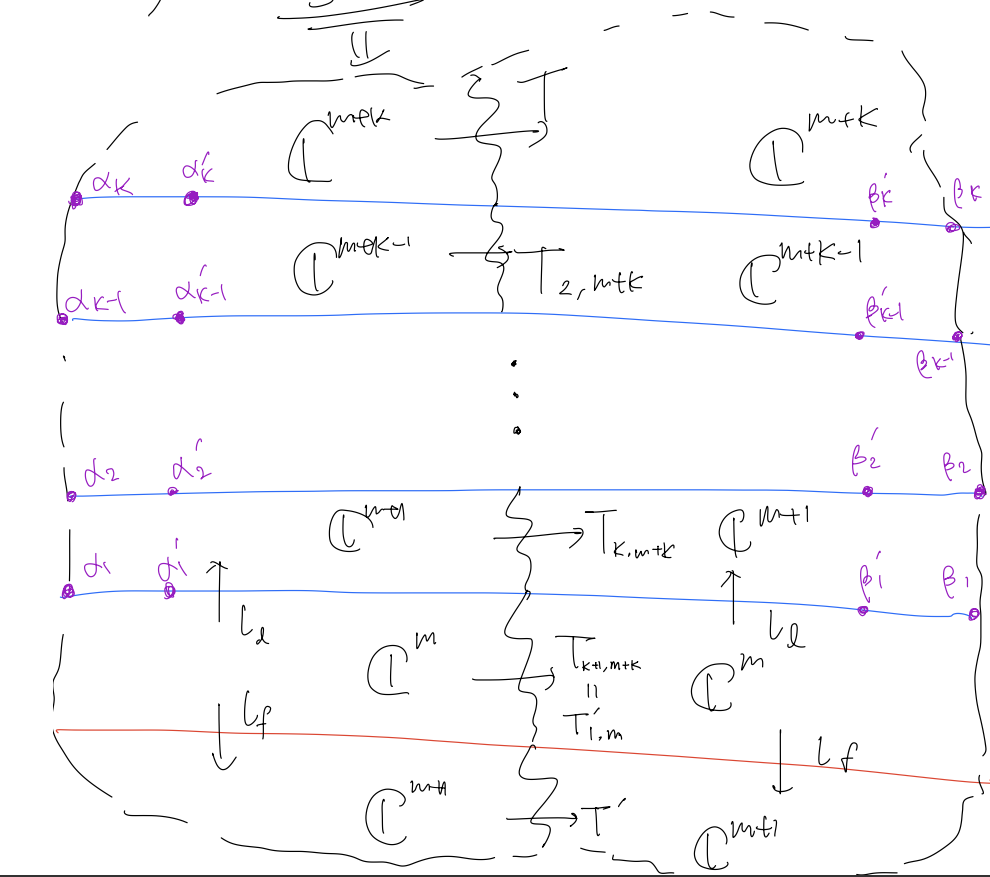
\includegraphics[width=\linewidth]{diagrams/lemma6/1.png} % Adjust the width as needed
    \caption{Your caption here}
    \label{fig:your-label}
\end{figure}
where $T$ is an isomorphism preserving the flag $\mathbb{C}^m\subset_l \mathbb{C}^{m+1}\subset_l\cdots\subset_l \mathbb{C}^{m+k}$(here $\subset_l$ denotes inclusion into the last factors), $T'$ is an isomorphism preserving $\mathbb{C}^m \subset_f \mathbb{C}^{m+1}$(here $\subset_f$ means inclusion into the first factors), and $T_{k+1,m+k}=T'_{1,m}$.

If we apply MOVE \RN{6} to the above diagram and the sheaf on it, we get the following:
\begin{figure}[H] % Optional: [h] means here, [t] for top, [b] for bottom, [p] for page of floats
    \centering
    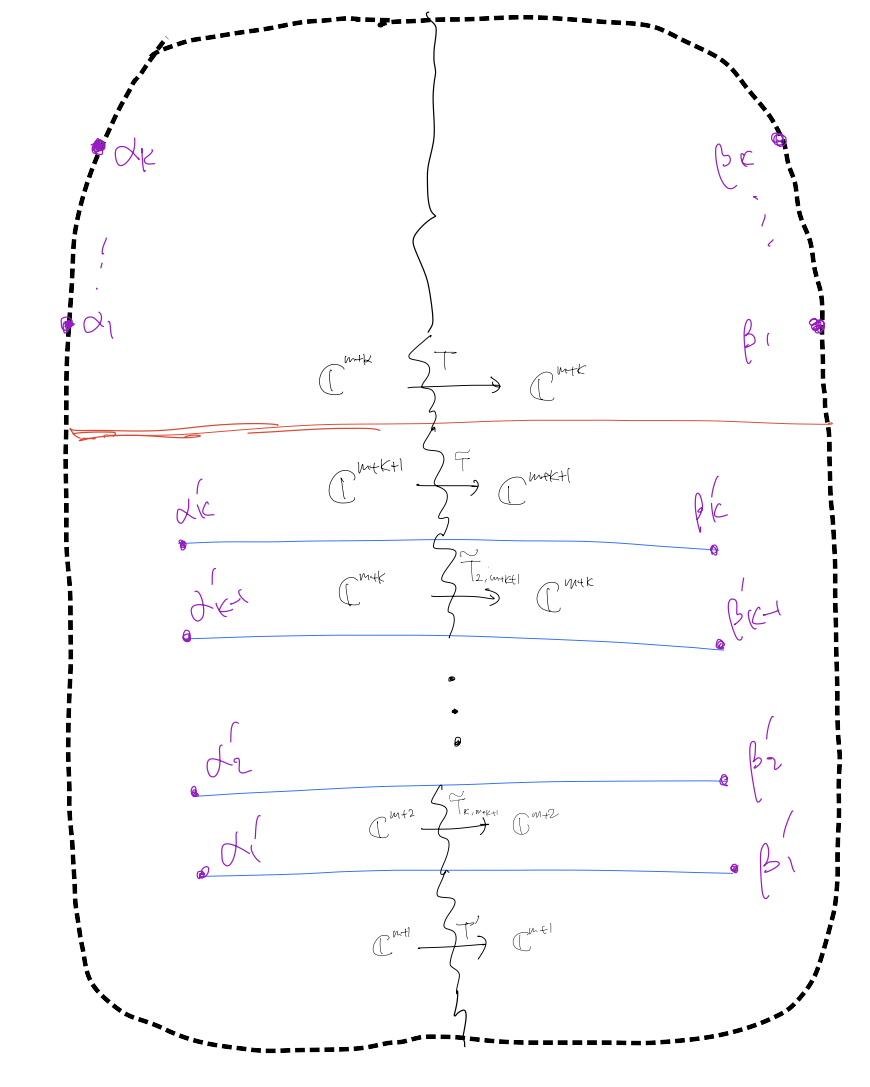
\includegraphics[width=\linewidth]{diagrams/lemma6/2.png} % Adjust the width as needed
    \caption{Your caption here}
    \label{fig:your-label}
\end{figure}
where $\tilde{T}_{1,m+k} = T$ and $\tilde{T}_{k+1,m+k+1} = T'$(rest of the entries are 0)

(proof) We prove the claim by induction on $k$. By the induction hypothesis after $k-1$ application of MOVE \RN{5}(MOVE \RN{6}), we get 
\begin{figure}[H] % Optional: [h] means here, [t] for top, [b] for bottom, [p] for page of floats
    \centering
    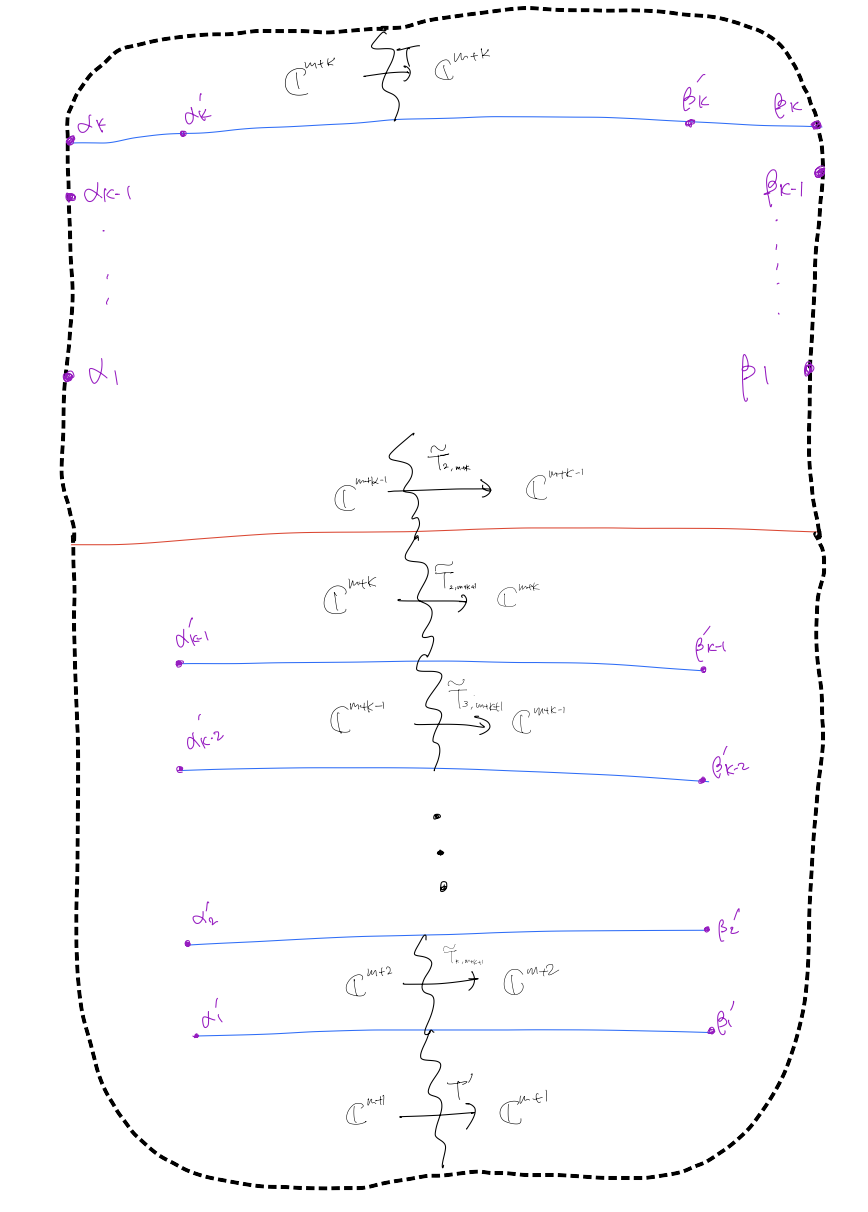
\includegraphics[width=\linewidth]{diagrams/lemma6/3.png} % Adjust the width as needed
    \caption{Your caption here}
    \label{fig:your-label}
\end{figure}

Now we apply MOVE \RN{5} to the uppermost blue strand and the red strand, then by Lemma5, we get

\begin{figure}[H] % Optional: [h] means here, [t] for top, [b] for bottom, [p] for page of floats
    \centering
    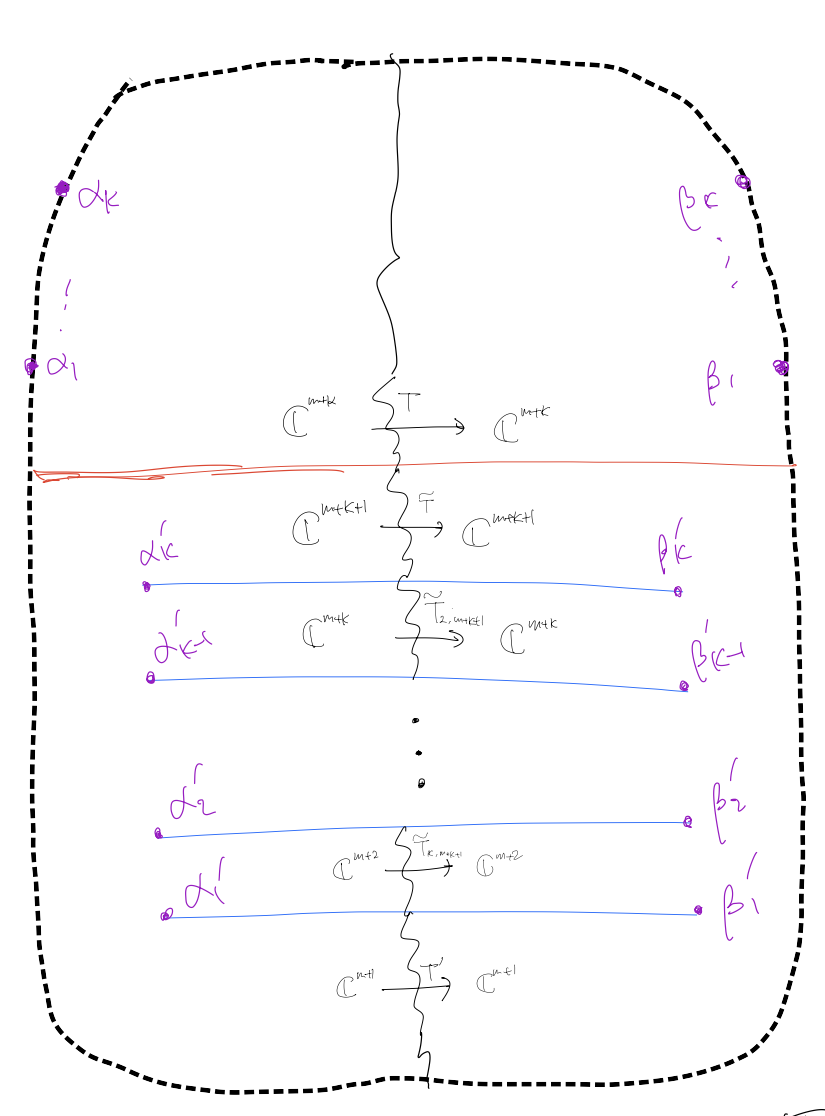
\includegraphics[width=\linewidth]{diagrams/lemma6/4.png} % Adjust the width as needed
    \caption{Your caption here}
    \label{fig:your-label}
\end{figure}